\documentclass[border=10pt]{standalone}
\usepackage{pgfplots}
\pgfplotsset{compat=1.18, trig format plots=deg}
\begin{document}
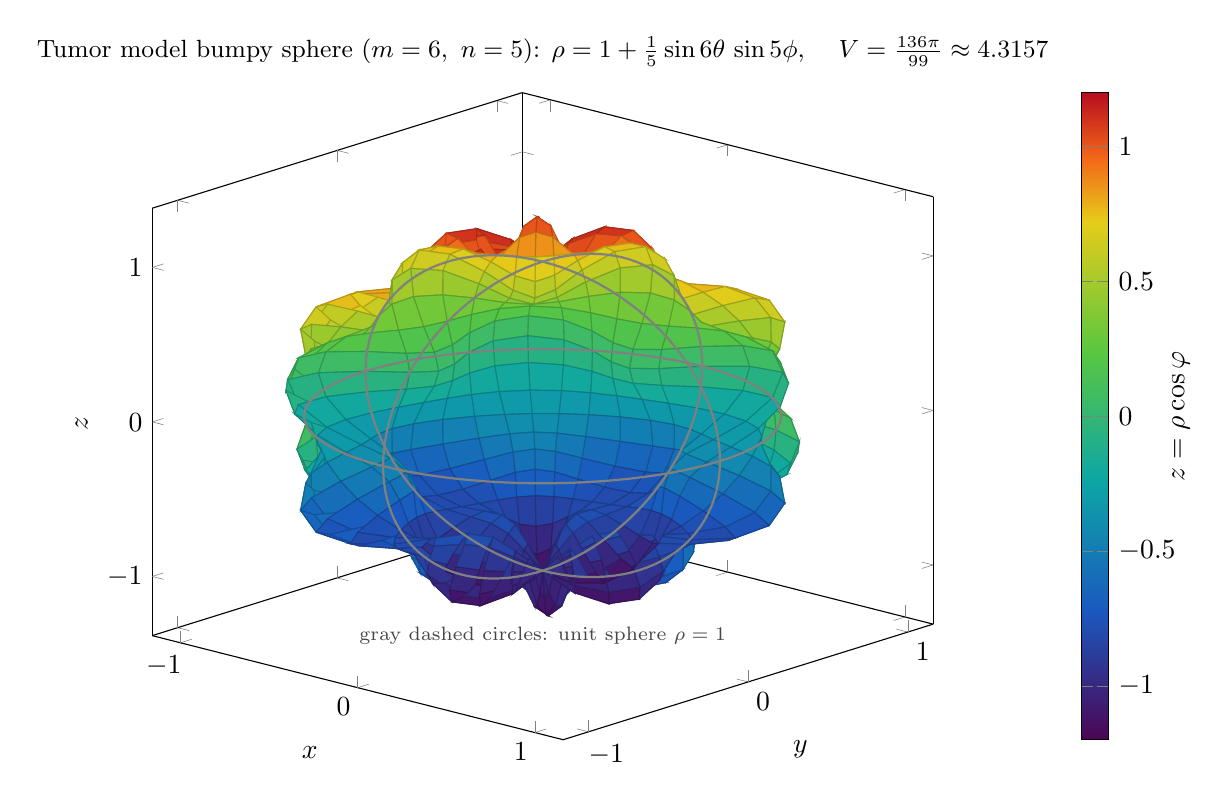
\begin{tikzpicture}
\begin{axis}[
    width=11.5cm, height=9.8cm,
    domain=0:360, y domain=0:180,
    samples=49, samples y=25,
    colormap={turbolike}{rgb(0cm)=(0.30,0.02,0.33); rgb(0.2cm)=(0.10,0.35,0.75);
                         rgb(0.4cm)=(0.05,0.65,0.65); rgb(0.6cm)=(0.35,0.78,0.25);
                         rgb(0.8cm)=(0.90,0.80,0.10); rgb(0.9cm)=(0.95,0.40,0.10);
                         rgb(1cm)=(0.72,0.05,0.12)},
    colorbar, point meta min=-1.2, point meta max=1.2,
    colorbar style={ylabel={$z=\rho\cos\varphi$}, ylabel shift=-8pt, width=0.35cm,
                    ytick={-1,-0.5,0,0.5,1}},
    view={42}{20},
    xlabel=$x$, ylabel=$y$, zlabel=$z$,
    xtick={-1,0,1}, ytick={-1,0,1}, ztick={-1,0,1},
    title={Tumor model bumpy sphere ($m=6,\ n=5$): $\rho=1+\frac{1}{5}\sin 6\theta\,\sin 5\phi$,
           $\quad V=\frac{136\pi}{99}\approx 4.3157$},
    title style={align=center, font=\small},
]
\addplot3[surf, shader=faceted]
  ({cos(x)*sin(y)*(1+0.2*sin(6*x)*sin(5*y))},
   {sin(x)*sin(y)*(1+0.2*sin(6*x)*sin(5*y))},
   {cos(y)*(1+0.2*sin(6*x)*sin(5*y))});
\addplot3[gray, dashed, thick, domain=0:360, samples=121] ({cos(x)},{sin(x)},{0});
\addplot3[gray, dashed, thick, domain=0:360, samples=121] ({cos(x)},{0},{sin(x)});
\addplot3[gray, dashed, thick, domain=0:360, samples=121] ({0},{cos(x)},{sin(x)});
\node[anchor=north, gray!55!black, align=center, font=\scriptsize] at (axis cs:0,0,-1.30)
  {gray dashed circles: unit sphere $\rho=1$};
\end{axis}
\end{tikzpicture}
\end{document}
